\chapter{Panel Interface Tester (PIT) additional notes for first contact latency measurement}
This appendix compliments the PIT documentation included in TPPT deliveries. It is related to first contact latency measurement. Figure \ref{fig:pit_robot_setup} shows in more detail the HW parts of PIT setup.

\begin{figure}[!h]
	\centering
	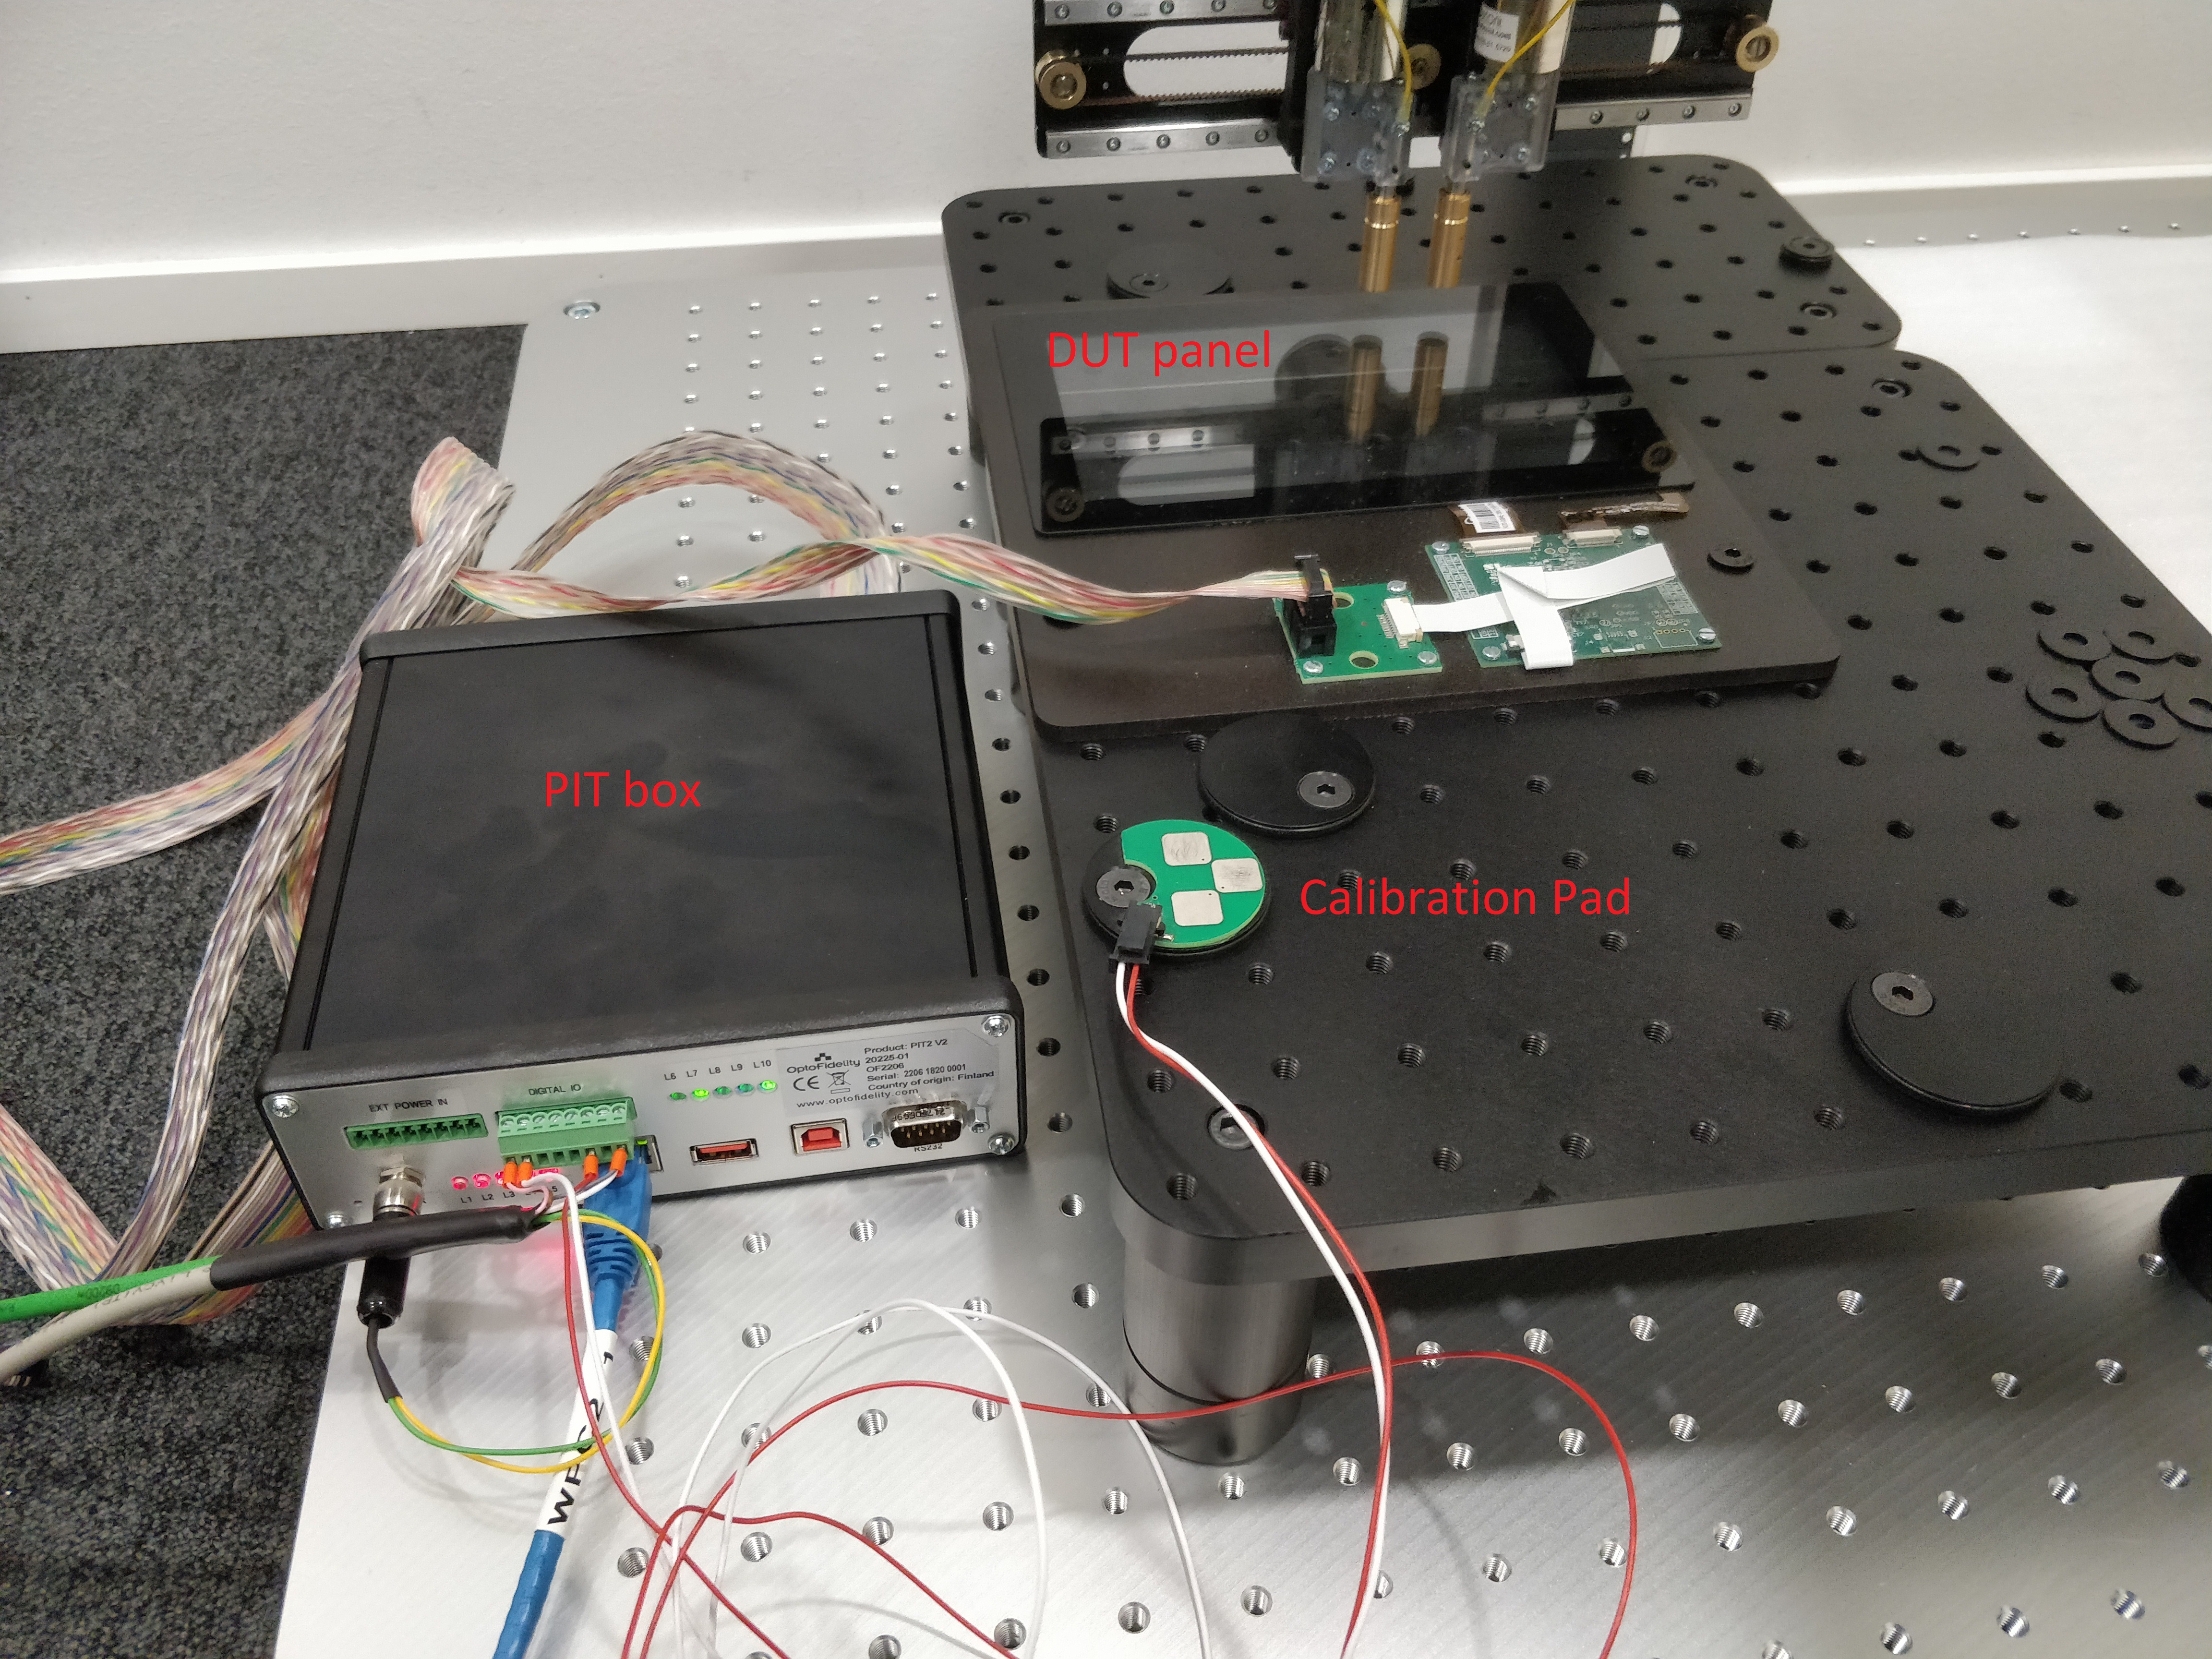
\includegraphics[width=0.7\linewidth]{pit_robot_setup.jpg}
	\caption{PIT robot setup.}
	\label{fig:pit_robot_setup}
\end{figure}

\section{Triggering options}
To measure first contact latency, the information of when the tool tip touches the DUT screen is needed. This is done via triggering. There are two options for this:
\begin{enumerate}
	\item Trigger signal based on voice coil encoder movement when moving down to DUT with Z-axis. This is the current standard solution. System latency calibration not needed with this option.
	\item Optical port attached to the fingertip. This is a legacy option used in older robots with no voicecoil. Requests system latency calibration.
\end{enumerate}


\section{System latency calibration}
\notebox{If voice coil triggering is used, the system latency calibration is not needed. It is typically around 2ms. The values may vary in different measurements between 0ms and 4ms being mainly 1-2ms. I.e., the values are really stable.}

System latency means the latency of the robot test system from the touch of the tip/finger to the moment timestamp is recorded, which is done inside PIT.

System latency can be calibrated when running First Contact Latency test:
\begin{itemize}
	\item "Calibrate system latency" selection in UI and configuration "hide\_system\_latency\_calibration" whether this is visible in UI.
	\item When running the calibration, you need to have special calibration pad connected to PIT2 box (see Figure \ref{fig:pit_robot_setup})
		\begin{itemize}
			\item Calibration pad must be positioned as DUT with name "OF\_PIT\_LATENCY" in TnT Server.
			\item Make sure top-left corner of the "OF\_PIT\_LATENCY" is on the metal area of the calibration pad. Calibration procedure taps very close to top left. So you shouldn't make top-left into the edge of one of the small metal areas but rather a bit towards the center of that area.
			\item Positioning accuracy doesn't really matter. Make it rather smaller than bigger so that calibration procedure taps the pad correctly.
		\end{itemize}
	\item System latency calculation:
		\begin{itemize}
			\item System latency = trigger timestamp - calibration pad timestamp.
			\item 10 taps are made and median of these is considered as the system latency.
			\item Calibration pad timestamp means the moment when finger touches calibration pad. This is routed electrically to PIT2 box and hence considered very accurate and instant.
			\item There is a small chance finger trigger is coming first if calibration pad trigger requires small pressure towards the pad. This has not realized but it's theoretically possible.
		\end{itemize} 
\end{itemize}



